\section{Problem 2}
\label{part2}
\subsection*{Question}
\begingroup
\begin{verbatim}
2.  Using your facebook account, repeat question #1 (if you have >
50 friends).

Start at: https://developers.facebook.com/docs/graph-api/reference/v2.1/user/friends

or perhaps:

http://socialnetimporter.codeplex.com/

\end{verbatim}
\newpage
\begin{enumerate}
\item After the second assignment I assumed that we should use API keys in order to get the data from any of the social networking sites. So I spend good amount of time in trying to figure out how to get the information by using these Keys and tokens
\item I registered for Facebook APP in order to get the API keys and wrote a piece of code to get the token. 
\begin{lstlisting}[frame=single]
from facepy import utils 
app_id = 14867915882649321
app_secret = "93595d85e282ce2bb395a21c921396312"
oath_access_token = utils.get_application_access_token(app_id, app_secret)
print oath_access_token
\end{lstlisting}
\item I tried using the library ``facebook'' but it did not work for me, so I shifted to facepy which worked fine for me. 
\item But I realized the token I am computing from the above python code is not what I need. I figured that the token I want is generated here \url{https://developers.facebook.com/tools/explorer/?method=GET&path=1310493851%3Ffields%3Dfriends&version=v2.1} and this expires every couple of hours. 
\item The python program \ref{lst:q2python} gives the list of my friends, but when I observed the output I see only 198 but in real I have 311 friends. By this observation it  is clear that I am getting the list of friends who are sharing their friends list.
\item When I tried to find the number of friends each of my friends have through the python program \ref{lst:q2python} I was shocked to see that the  result came up for only 3 of my friends. And for others I get an error``Unsupported Operation''.
\item After some research I understood that through tokens we can not get full data from the Facebook profile, the friend count can only be retrieved for those friends who have registered for developer account and allowed access to their friend list.
\item So I ended up using the code \ref{lst:q2fbpython} ALEX had shared in the group to get the friend count. I retrieved friend count of each of my friends. 
\item The output for the code \ref{lst:q2fbpython} is not formatted. So I wrote a piece of code to format it as I want it. The code is listed in\ref{lst:q2fbsort}
\item I sorted the output retrieved from program \ref{lst:q2fbsort} by a simple command in Linux 
\begin{lstlisting}[frame=single]
 sort -n -k1 facebook.txt > fbSorted.txt
\end{lstlisting}
\item seeing as I am only person with 311 friends on my circle, it was easy to color the single bar with red color using the code on lines 11 and 12 in listing \ref{lst:q2Rbarplot}.
\item some friends do not share their friends counts, so they are left out of the data collected.
\item The median, Standard Deviation and mean is calculated by using the code on lines 
4,5 and 6.
	\begin{itemize}
		\item Mean:  487.505050505051
		\item Median:  409.5
		\item Standard Deviation:  389.037217791762
	\end{itemize}
	
\item I tried plotting the graph in scatter plot but I liked the bar plot better.
\end{enumerate}
\newpage
\lstinputlisting[language=python, frame=single,breaklines=true, caption={Python program for getting the list of Friends by using facepy}, label=lst:q2python, captionpos=b, numbers=left, showspaces=false, showstringspaces=false, basicstyle=\footnotesize]{fb/getmyfrnds_fb.py}
\newpage

\lstinputlisting[language=python, frame=single,breaklines=true, caption={Python program for getting the list of Friends by using selenium}, label=lst:q2fbpython, captionpos=b, numbers=left, showspaces=false, showstringspaces=false, basicstyle=\footnotesize]{fb/seleniumScrapePB.py}
\newpage
\lstinputlisting[language=python, frame=single,breaklines=true, caption={Python program for formatting the list}, label=lst:q2fbsort, captionpos=b, numbers=left, showspaces=false, showstringspaces=false, basicstyle=\footnotesize]{fb/facebook_sort.py}
\newpage
\lstinputlisting[language=R, frame=single,breaklines=true, caption={R script for bar plot shown in Figure \ref{fig:q2-1} }, label=lst:q2Rbarplot, captionpos=b, numbers=left, showspaces=false, showstringspaces=false, basicstyle=\footnotesize]{fb/barplotFb.R}

\begin{figure}
	 \begin{center}
		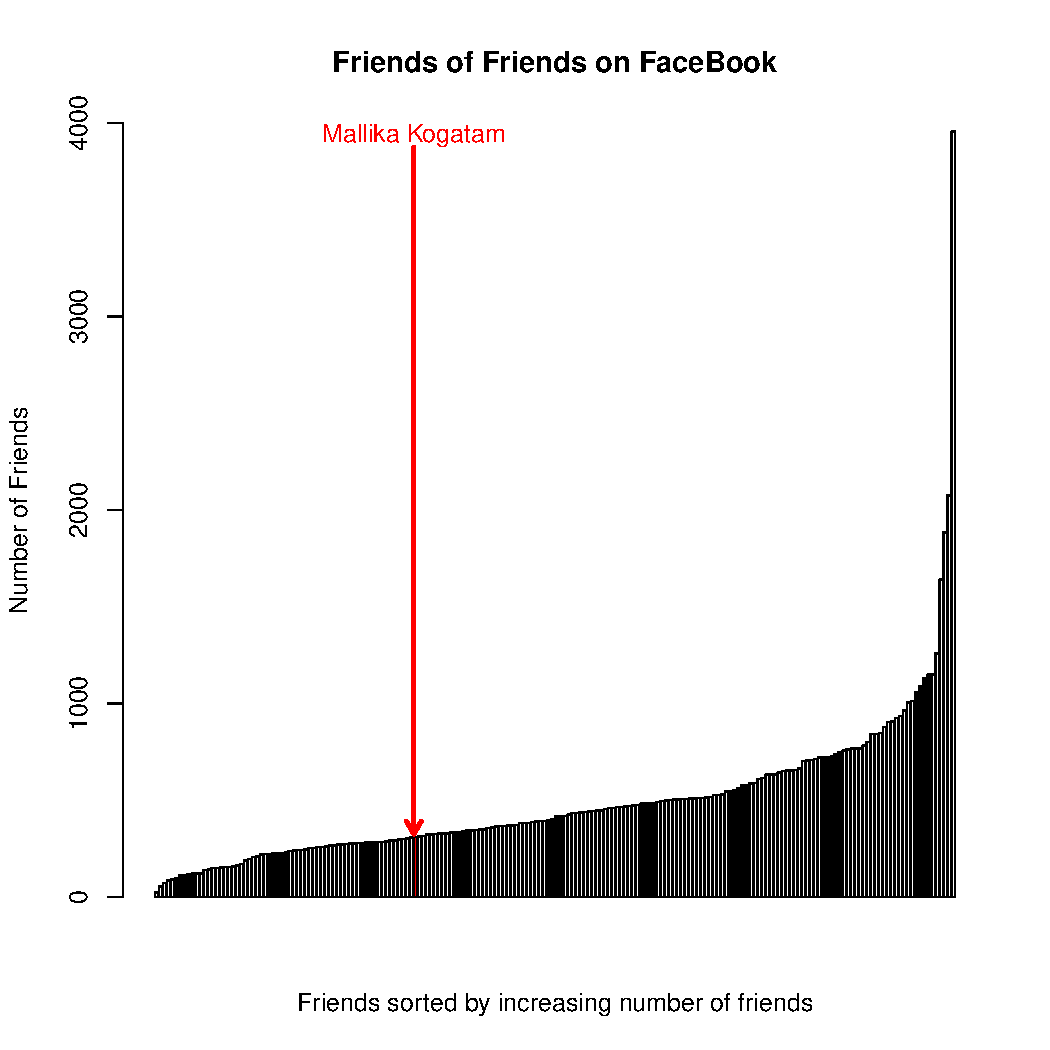
\includegraphics[scale=0.8]{fb/fb_barplot.pdf}
		\caption{BarPlot for no of friends and the friends sorted by number of friends}
		\label{fig:q2-1}
 	\end{center}
\end{figure}